\documentclass[a4paper,11pt]{article}

% 日本語対応
\usepackage{xeCJK}
\setCJKmainfont{Yu Gothic}

% 数学関連パッケージ
\usepackage{amsmath}
\usepackage{amssymb}
\usepackage{amsthm}
\usepackage{amsfonts}
\usepackage{mathtools}

% 図形描画用パッケージ
\usepackage{tikz}
\usepackage{pgfplots}
\pgfplotsset{compat=1.18}
\usetikzlibrary{intersections,patterns,angles,quotes,calc,fillbetween}

% その他パッケージ
\usepackage{graphicx}
\usepackage{enumitem}
\usepackage{float}
\usepackage{hyperref}
\usepackage{fancyhdr}
\usepackage{geometry}
\usepackage{xcolor}

% ページ設定
\geometry{
  a4paper,
  top=25mm,
  bottom=25mm,
  left=25mm,
  right=25mm
}

% 数式環境設定
\numberwithin{equation}{section}
\newtheorem{theorem}{定理}
\newtheorem{lemma}[theorem]{補題}
\newtheorem{proposition}[theorem]{命題}
\newtheorem{corollary}[theorem]{系}
\theoremstyle{definition}
\newtheorem{definition}[theorem]{定義}
\newtheorem{example}[theorem]{例}
\newtheorem{exercise}{問題}
\theoremstyle{remark}
\newtheorem*{remark}{注意}
\newtheorem*{solution}{解答}

% ヘッダーとフッターの設定
\pagestyle{fancy}
\fancyhf{}
\fancyhead[L]{数学問題}
\fancyhead[R]{\today}
\fancyfoot[C]{\thepage}
\renewcommand{\headrulewidth}{0.4pt}
\renewcommand{\footrulewidth}{0.4pt}

% タイトル情報
\title{数学問題}
\author{数学問題生成AIシステム}
\date{\today}

% ドキュメント開始
\begin{document}

\maketitle

% 問題セクション
\section*{問題}

% 問題文を挿入(変数で置換)
2次関数 $f(x) = 2x^2 - 4x + 3$ の頂点の座標を求めるには、頂点の公式を使用します。頂点の$x$座標は、$x = -\frac{b}{2a}$ で求められます。ここで、$a = 2$、$b = -4$ です。したがって、

\[x = -\frac{-4}{2 \cdot 2} = \frac{4}{4} = 1\]

次に、この$x$の値を元の関数に代入して、$y$の値を求めます。

\[y = 2(1)^2 - 4(1) + 3 = 2 - 4 + 3 = 1\]

したがって、頂点の座標は $(1, 1)$ です。

% 図形が必要な場合はここに挿入
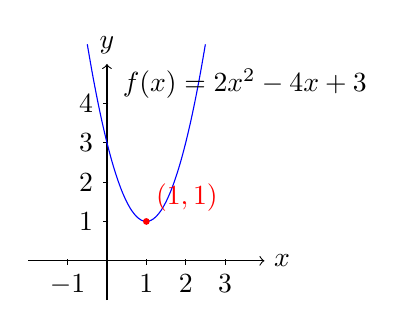
\begin{tikzpicture}[scale=0.5]
  % Draw axes
  \draw[->] (-2,0) -- (4,0) node[right] {$x$};
  \draw[->] (0,-1) -- (0,5) node[above] {$y$};
  
  % Labels
  \foreach \x in {-1,1,2,3}
    \draw (\x,1pt) -- (\x,-3pt) node[anchor=north] {$\x$};
  \foreach \y in {1,2,3,4}
    \draw (1pt,\y) -- (-3pt,\y) node[anchor=east] {$\y$};
  
  % Draw function
  \draw[domain=-0.5:2.5,smooth,variable=\x,blue] plot ({\x},{2*\x*\x - 4*\x + 3});
  
  % Draw vertex
  \filldraw[red] (1,1) circle (2pt) node[anchor=south west] {$(1,1)$};
  
  % Function label
  \node at (3.5,4.5) {$f(x) = 2x^2 - 4x + 3$};
\end{tikzpicture}

% 解答セクション(オプショナル - 表示したくない場合はコメントアウト)
\section*{解答}

% 解答を挿入(変数で置換)
$(1, 1)$

% 解説セクション(オプショナル - 表示したくない場合はコメントアウト)
\section*{解説}

% 解説を挿入(変数で置換)
二次関数 $f(x) = ax^2 + bx + c$ の頂点の座標は、$\left(-\frac{b}{2a}, f\left(-\frac{b}{2a}\right)\right)$ である。ここで $a = 2$, $b = -4$, $c = 3$ となるため、$-\frac{b}{2a} = -\frac{-4}{2\cdot2} = 1$ である。したがって、$x = 1$ のときの $f(x)$ の値を求めると、$f(1) = 2\cdot1^2 - 4\cdot1 + 3 = 2 - 4 + 3 = 1$ となる。従って、頂点の座標は $(1, 1)$ となる。

\end{document} 